\paragraph{}
Figure \ref{img:secur} describes how a customer deals with
AlSpark in order to implement a security system in their 
enterprise.
The workflow is divided into three phases, the first regards
requirements analysis: here the customer can purchase some 
hardware devices which are needed in order to complete the
system.

Then, during the developing phase, AllSpark releases periodically
a beta version of the system, which will be tested with the customer's
support in order to fine-tune the requirements.

Finally when the system is completely operative, AllSpark install
the definitive version on the customer machines. 

\paragraph{}
In figure \ref{img:certs} is described the procedure followed for
taking part in formation courses in order to take certification of
quality as sysadmin or developer.

The AllSpark policy regarding the courses is that a customer has 
two possibility of taking the exam each time he subscribes to the
course. 

\begin{figure}
\centering
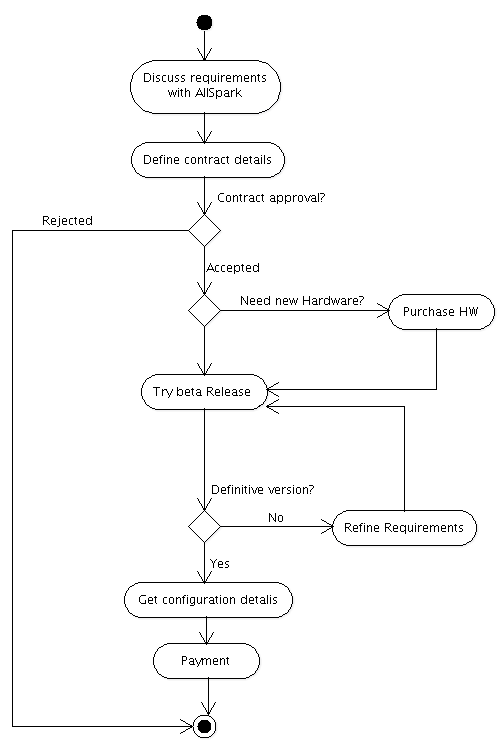
\includegraphics[scale=0.70]{argouml_diags/imgs/secur}
\caption{Workflow of project development}
\label{img:secur}
\end{figure}

\begin{figure}
\centering
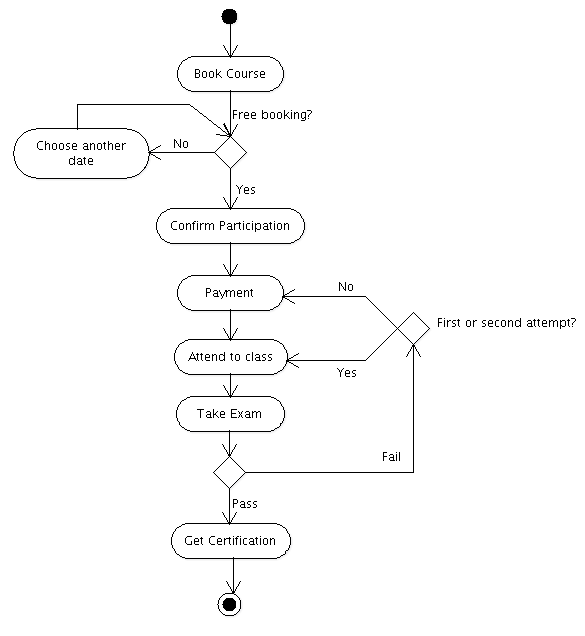
\includegraphics[scale=0.75]{argouml_diags/imgs/certs}
\caption{Procedure followed for getting certifications}
\label{img:certs}
\end{figure}

